\chapter{Quantitative methods for social research in the digital age}

Quantitative social scientists often attempt to understand the
behavior of political entities, and digital records are one of the
most useful resources available to them.  The digital age has brought
to these researchers a deluge of records---particularly in the
form of text.  This avalanche of data provides more information to
these scientists than they have had in the history of mankind.

Researchers are now able to pore over digital copies of all legally
binding opinions written by United States Supreme Court Justices, or
the text of thousands of bills voted on by members of Congress.  Even
these numbers are dwarfed by the hundreds of thousands of newspaper
articles and blog posts written each day about the events happening in
the world.  Unfortunately, this flood of information obscures the very
insights these researchers aim to discover.  Researchers trying to
make sense of these collections are subject to the high costs of time
spent poring over these collections in search of the few key insights.

 % example questions: how to find phenomena in collections of text
 % how to 
% The goal of this thesis is to demonstrate that complex, meaningful patterns of
% information can be gleaned
% Society interacts with this information in
% a complicated dance: information affects what we do, and we create
% further information -- books, scientific papers, legislation, and
% tweets -- as a result.  Information influences everything we say,
% think, and do.
The goal of this thesis is to describe several new statistical models
that are now available for data practitioners and the consumers of that
data\footnote{By a (data) practitioner, I am referring to anyone who
  applies existing methods for data analysis, possibly tweaking or
  combining these methods to answer specific questions (such as
  database engineers or lab assistants). This contrasts with
  fundamental researchers, who research entirely new methods or tools
  for data analysis.  A social scientist may be a researcher
  in his or her field but a practitioner in the field of data
  analysis.} to better understand society through collections of
text documents.  I will focus on four high-level research questions
that dovetail off one another to illustrate the flexibility and
interpretability of latent variable models in large-scale settings.

An implicit premise of this thesis is that patterns are ubiquitous in
collections of text documents, and that these patterns can be
discovered automatically to describe decisions and behavior of actors
in these collections.  I will ground this discussion with the
development of several specific statistical models, but I will stress
throughout this thesis that these methods frequently draw from a suite
of common tools which can be used again and again to construct models.

\section*{The deluge of information and some statistical tools}

% The availability of observational social science data on a massive scale
Observational social science data -- including data about how
organizations and the Government work -- has become available on a
massive scale. The National Archive, which collects information from
over 500 federal agencies, has been digitizing its collection of
twelve \emph{billion} federal documents \citep{lazer:2009,
  national_archives:2012a,national_archives:2012b}.  The problem in
handling this data has moved from collecting the data to processing
and understanding it.  Fortunately for scholars, these data follow
recurring patterns which make statistical modeling possible. In this
thesis, I will focus on three specific patterns:

\paragraph{Text data.} Text data is the low-hanging fruit of most
social science research questions.  It is ubiquitous because it
can---indeed, it must---be easily created, digitized, and stored. Text
data serve as an observation which we can use to better understand the
story underlying decisions and politics.

Just as text data is invaluable to researchers, the rate of growth of
these text collections is staggering.  A single newspaper like the
\emph{New York Times} publishes hundreds of thousands of articles each
decade.  Of the National Archive's collection, billions of its
documents are text
\citep{national_archives:2012a,national_archives:2012b}.  The rate of
growth of sources like the World Wide Web is even more tremendous.  As
far back as 2008, the Internet was already growing at a rate of
several billion webpages per \emph{day} \citep{googleblog:2008}.

\paragraph{Time-series collections.}  Many datasets comprise
time-series observations.  Timestamps are one of the simplest types of
metadata to attach to digital collections because they are described
by a single scalar and because they are inexpensive and widely
available.  In spite of its simplicity, the addition of a time
variable to statistical models can provide rich insight and a useful
historical perspective into collections of documents.  It is
especially interesting to researchers because it is helpful in framing
questions about causation, prediction, and influence.

\paragraph{Relational observations.}
One of the simplest ways to represent more complicated phenomena is to
use the interaction between pairs of items.  We will refer to such
pairs (and their relationships) as \emph{dyadic}. In later chapters we
will use spatial models to represent interactions between lawmakers
and bills (i.e., how congresspersons voted on bills) and between
countries (i.e., countries' sentiment toward one another).  As we will
show, the underlying representation for these cases is very similar.

\subsection*{The role of statistical machine learning}

The deluge of information available to researchers means that if
researchers want broad coverage over the available sources, they
cannot spend long looking over any single document.  For example, a
graduate student studying patterns governing the relationships between
pairs of countries, based on mentions of pairs of countries in the
last twenty years of the \emph{New York Times}, would need to spend
every day of an entire year, twenty-four hours per day, to code the
300,200 interactions per pair of countries (at two minutes per
article).  A \emph{computational} treatment is therefore necessary if
researchers intend to handle large collections of data.

% In each of the models we will consider, the basic unit of analysis
% lives in an extremely high-dimensional space.  For example, treating
% text documents as bags of words still leaves the researcher with
% thousands of dimensions, and lawmakers described by their votes are
% still described by these thousands of dimensions.  In addition to
% text, another recurring theme in this thesis is that these
% high-dimensional observations can be described by much
% lower-dimensional summaries without losing much of the relevant
% information.

Statistical representations of these data will be useful because they
provide an explicit way to formalize our assumptions.  We are
fortunate that computers can be programmed to speak in this language,
because they are the only means by which we can achieve broad
understanding of large collections of text documents.

In this thesis, I will use probabilistic models to encode these
statistical assumptions.  I will frequently use the paradigm of
graphical models \citep{pearl:1985} to encode and describe our
assumptions.  Because these statistical methods provide directed
summaries, they can serve as optical lenses for researchers to analyze
entire collections of documents, which I illustrate as a cartoon in
\myfig{person_data_lens}.  Statistical methods enable researchers to
describe arbitrarily complex transformations of data with arbitrarily
complex lenses.  Because of the simplicity of each of these lenses,
we will find that a wide array of models can be created by nesting and
re-using modules across different applications.

\begin{figure}
  \center
  \begin{tabular}{ccc}
    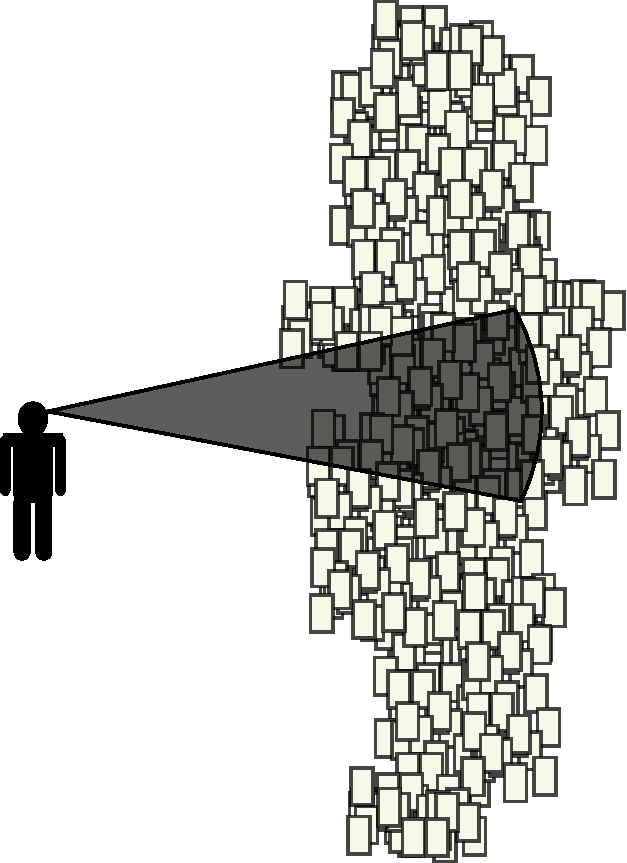
\includegraphics[width=0.3\textwidth,height=0.3\textwidth]{chapter_introduction/figures/person_data.pdf} &
    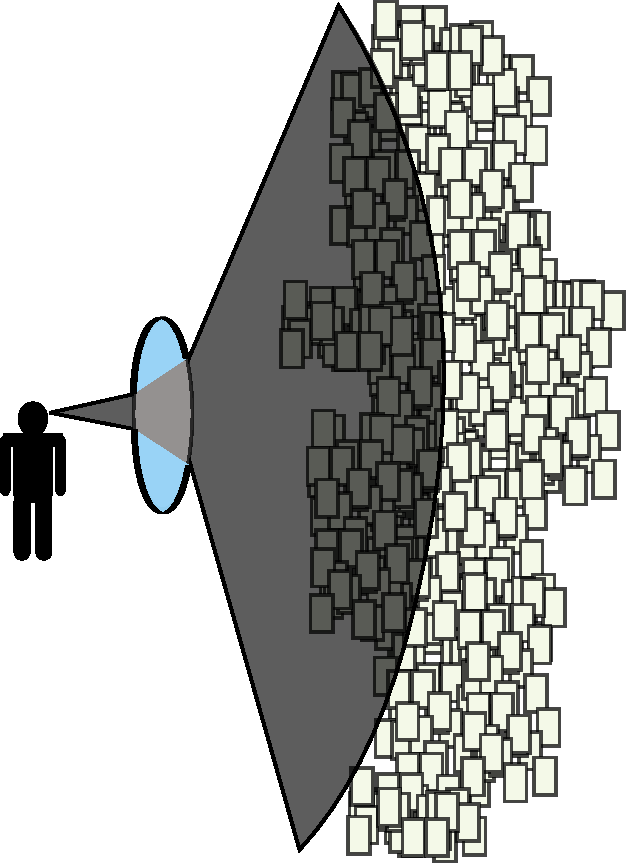
\includegraphics[width=0.3\textwidth,height=0.3\textwidth]{chapter_introduction/figures/person_data_lens.pdf} &
    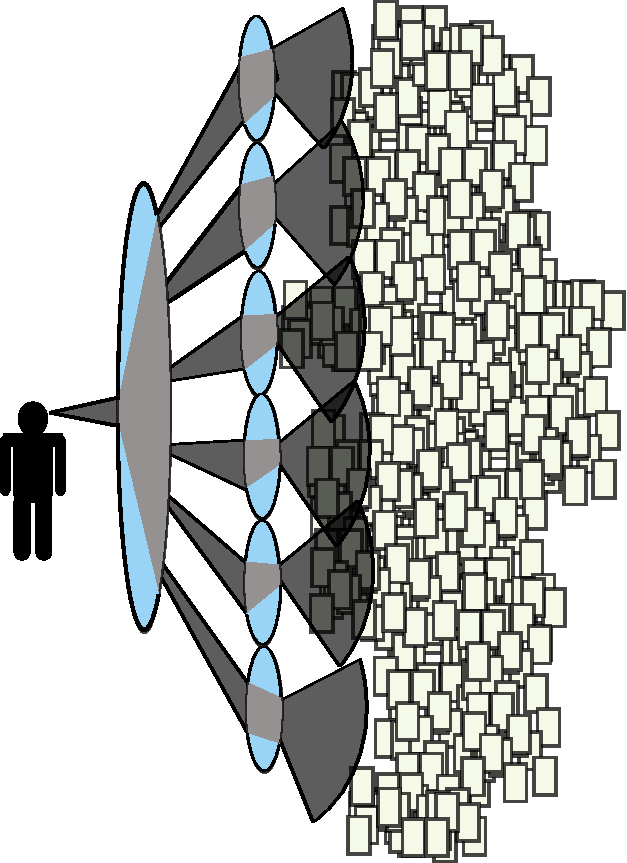
\includegraphics[width=0.3\textwidth,height=0.3\textwidth]{chapter_introduction/figures/person_data_lens2.pdf} \\
  \end{tabular}
  \caption{A cartoon illustration of the role of statistical models in
    large-scale data analysis.  Left: large data collections are too
    large to handle without special tools. Center, Right: statistical
    models serve as lenses which can be nested, adjusted, and
    custom-designed to glean latent structure from large or complex
    datasets.  Our statistical assumptions define the shape and
    optical characteristics of these lenses, and fortunately many of
    these lenses can be re-used.}
  \label{fig:person_data_lens}
\end{figure}

% - Tools and abstractions for probabilistic inference

\section*{Organization}

By the end of this thesis, the reader should have a better
understanding of several new models that I have designed for to social
scientists.  Perhaps more importantly, the reader will be prepared to
design his or her own latent-variable model for similar applications.

To this end, I will provide a lower level of detail about
latent-variable models in the early chapters of this thesis than
normally expected in a doctoral thesis when it may help a reader
unfamiliar with this subject to understand the material.  I also
present some of the most advanced (or uninteresting) math in the
appendix to keep the discussion of applications and modeling at the
forefront.

I provide preliminary material in Chapter 2, outlining the statistical
``primitives'' that I will use as building blocks in later chapters:
tools for working with text data, time-series data, and dyadic data.
This chapter also provides a high-level introduction to the algorithms
we will use for Bayesian inference.

\paragraph{Identifying influential documents.} After introducing the
foundations of this thesis, I begin with a question about the broad
strokes painted by a document collection. In \mychap{influence}, I
look at a common challenge in analyzing text collections: that of
finding the most important and influential documents in a corpus which
has grown over time.  This is a challenge in understanding collections
of academic articles, legal opinions, email archives, and many other
collections. This question even motivated the algorithm behind Larry
Page and Sergey Brin's PageRank algorithm, which recursively measures
the influence of Webpages, as measured by the hyperlinks between
Webpages \citep{garfield:1992,brin:1998,garfield:2002}.  Unlike Web
pages and academic articles, of course, explicit citations or
hyperlinks are unavailable, and researchers only see the most basic
metadata: documents' timestamps.  To this end, I will introduce a
model for discovering the most influential documents in such a
collection. I will validate this model on a set of several datasets,
including several collections of academic articles and a set of
opinions written by judges in the New York Appellate Courts system.

\paragraph{Inferring history from a collection of newspaper articles.}
In \mychap{foreign_relations} I will zoom in a bit to consider the
story within a collection of documents and outline a model to better
understand the relationships between pairs of countries over time.  I
will fit this to a collection of \emph{New York Times} articles and
demonstrate that this method discovers a more sophisticated latent
story among documents than in Chapter 3.  As with the method in Chapter
3, this collection has only the text of these articles, which I
augment with external information.  In this chapter I also incorporate
important ideas from the field of dyadic spatial models, which can
play a role in modeling various social science phenomena.

% I will describe a method to discover
% which documents are influential on the development of a collection of
% text documents \emph{without} the use of metadata such as
% citations---where by an ``influential'' document I mean one that uses
% language which is adopted by others in the collection.

\paragraph{Inferring lawmakers' preferences.}

In Chapters~\ref{chapter:predicting_votes}
and~\ref{chapter:issue_adjustments} I will take an even closer look at
how documents can be used to better understand how congresspersons vote on
bills.  I will address two important limitations of ideal point models
(the state of the art in spatial voting models) by using the text of
bills.  One of these limitations is that ideal points cannot be used
to predict lawmakers' votes on heldout bills.  In
\mychap{predicting_votes}, I will introduce several models for
predicting votes by lawmakers on previously-unseen bills.  I will
demonstrate that we can predict lawmakers' votes with high accuracy
given their prior voting record and the text of the bills on which
they vote.

In \mychap{issue_adjustments} I will address a second shortcoming of
ideal point models: the limitation of a one-dimensional latent space.
I will do this by using a topic model to identify those issues up for
vote in an item of legislation.  I will demonstrate that legislators'
votes can be better modeled and better understood by describing these
lawmakers' positions on different issues.

These models contrast with those in Chapters 3 and 4 in that I ignore
documents' timestamps.  However, I will use many of the same ideas
from these earlier chapters, including mixed-membership models of text
and latent-space models, in which I assume that pairs of items
interact (in this case a lawmaker and a bill), and that text documents
attached to those interactions can provide insight into the
interaction.

\paragraph{Additional materials.}
In Appendix~\ref{chapter:stochastic_variational_optimization} I
discuss details of a new variational inference algorithm which is used
in \mychap{issue_adjustments}.  This Appendix can be treated as a
stand-alone contribution of this thesis, making a quantitative rather
than a substantive contribution.  I save this contribution for the
appendix in part to stress my fundamental belief that model
development and model implementation can be treated separately (or
should be treated as separate whenever possible to enable
practitioners to do their magic), and because I believe that this
thesis will appeal more broadly if it is not bogged down with
mathematical baggage.  I provide additional supplementary information
for the remaining chapters in
Appendix~\ref{chapter:supplementary_materials}.
